\documentclass[11pt, a4paper]{article}

\usepackage[utf8]{inputenc}
\usepackage[italian, english]{babel}
\usepackage[pages=some]{background}
\usepackage{hyperref}
\usepackage{amsmath}
\usepackage{subcaption}


\graphicspath{ {./img/} }
\backgroundsetup{
	firstpage = {true},
	placement = {center},
	position = current page.center,
	contents = {
\includegraphics[scale=0.07]{unipd}},
	angle = {0},
	opacity = {0.03}
}
\hypersetup{
	colorlinks=true,      
	urlcolor=blue,
	linkcolor=black
}

\title{Vision and Cognitive Services\\
\large Video Frame Interpolation via Adaptive Separable Convolution}
\author{Filippo Visentin (2020581)\\
Nicola Carlesso (1237782)}
\date{a.a. 2020/2021}

\begin{document}
	\pagenumbering{gobble}
	\maketitle
	\clearpage
	
	\tableofcontents
	\clearpage
	\pagenumbering{arabic}
	
	\section{Introduction}
	Our work is related on the video frame interpolation problem. In particular we look at work in \cite{mainpaper}; when we talk about ``our network'', we refer to a modified version of the network in \cite{mainpaper}.\\
	The video frame interpolation problem consists of recreating the frame between two input frames in a video. This problem allows either to obtain a higher quality video, in terms of frames per second, a more defined slow motion, or a super slow motion.\\
	The main challenge of this problem is to get an output frame with defined shapes, because the network tends to give in output a blurred frame, and recreate a good frame in case the two input frames are quite different.\\
	Our network has a decoder-encoder architecture, used mainly to recreate fake examples from a dataset, as in our case study. The network doesn't create directly the interpolated frame, but gives in output an ad hoc couple of kernels (separable kernels) for each input frame. As last step we apply the convolutional operation with output kernels and input frames to get the output frame. 
	
	\section{Related work}
	Other approaches to solve this problem use the optical flow technique \cite{optical_flow}, where the network learns movements of figures in the frame and predicts those immediately following. This technique requires two main steps: first estimate optical flow between input frames and then synthesize an intermediate frame guided by motion; our approach requires instead a single convolution.\\
	The work we rely on is a continuation of another work in \cite{previous_work} that use our same network structure with one, mainly difference: in our network we obtain two separable kernels for each input frame, a column and a row vector, in \cite{previous_work} the network gives in output one ``standard'' kernel (a square matrix) for each input frame. This difference gives a big improvement in terms of memory and computational time, in fact the usage of memory went from 26GB to 1.27GB.  In this way, an $n \times n$ convolution kernel can be encoded using only $2n$ variables.\\
	Another improvement is the sharpness and quality of output frames.
	
	\section{Dataset}
	Fortunately, for the video frame interpolation problem, it's easy to create a large dataset without looking online.\\
	We just have to take a video and extract a triplet of close frames. The input are the first and last frame of triplet, and the label is the second frame. It's important consider two factors:
	\begin{itemize}
		\item all frames in triplet must be enough different, otherwise the example will be useless for the learning phase;
		\item all frames in triplet don't must be too much different. For example, in the case of in the middle of triplet a change of scene occurs. 
	\end{itemize}
	Therefore, we analysed the difference of image histograms of triplet's frames to have the magnitude of motion and then we compared them by taking the norm of the difference vector, setting lower and upper bound.\\
	Another important hyper-parameter used to create the database is the number of frames between elements of the triplet. In this way we have examples that can show more os less movement, to test the strength of network. To create our dataset we use \href{https://www.crcv.ucf.edu/data/UCF101.php}{UCF-101}.\\
	With all videos in UCF-101, we can get about 500'000 examples. Unfortunately, already with 150'000 examples and a \textit{batch size} of 32 examples, an epoch requires about 1000 seconds of time, so we used for our experiments a dataset of 50'000 examples (we note that using 50'000 or 75'000 examples, the results don't change too much).
	 
	\section{Method}
	Our structure of CNN is based on that of \cite{mainpaper}, showed in Figure~\ref{original-net}, with some changes. At the core there is a encoding phase with 6 steps of 3-stack of convolutional layers, separated by average pooling layers. The decoding phase is the reverse of previous, with a bilinear upscaling. The upscaling reintroduces feature maps from the encoding layer, in order to facilitate the decoding. As output of the network we expect a couple of separable kernels for each pixel, used to combine pixels from the two input frames to obtain each new pixel of the interpolated frame. The skip connection technique is used, to let the expanding layers incorporate features from the contracting part of the neural network.\\
	We call $I_1$ and $I_2$ two input frames and $\hat{I}$ the interpolated frame to compute each output pixel $(x,y)$. In the final stage applies at each input frame a convolutional operation between every output kernel and patches centred in $(x,y)$.\\
	As we ca see in Figure~\ref{original-net}, if we consider inputs like a matrix $128\times128$ and we set the size of separable kernels as $51\times1$, the output of network (with batch size of 1) are four matrices $128\times128\times51$: $k_{1,h}$, $k_{1,v}$, $k_{2,h}$, $k_{2,v}$; hence $k_{n,s}(x,y)$ is a vector $51\times1$.\\
	For the last step, given the output of network, we call $K_n(x,y) = k_{n,h}(x,y) \cdot k_{n,v}(x,y)$, a matrix $51\times51$, and the input patch centred in $(x,y)$ of \textit{n-th} input frame $P_n(x,y)$, always a matrix $51\times51$.\\
	Each output pixel $\hat{I}(x,y)$ is calculate using the Equation~\ref{eq} (``$*$'' represents the point-wise multiplication plus the sum of matrix's values). We can observe that when we make this operation for each pixel, we obtain the convolutional operation. 
	
	\begin{equation}
		\hat{I}(x,y) = K_1(x,y) * P_1(x,y) + K_2(x,y) * P_2(x,y)
		\label{eq}
	\end{equation}
	
	\begin{figure}
		\centering
		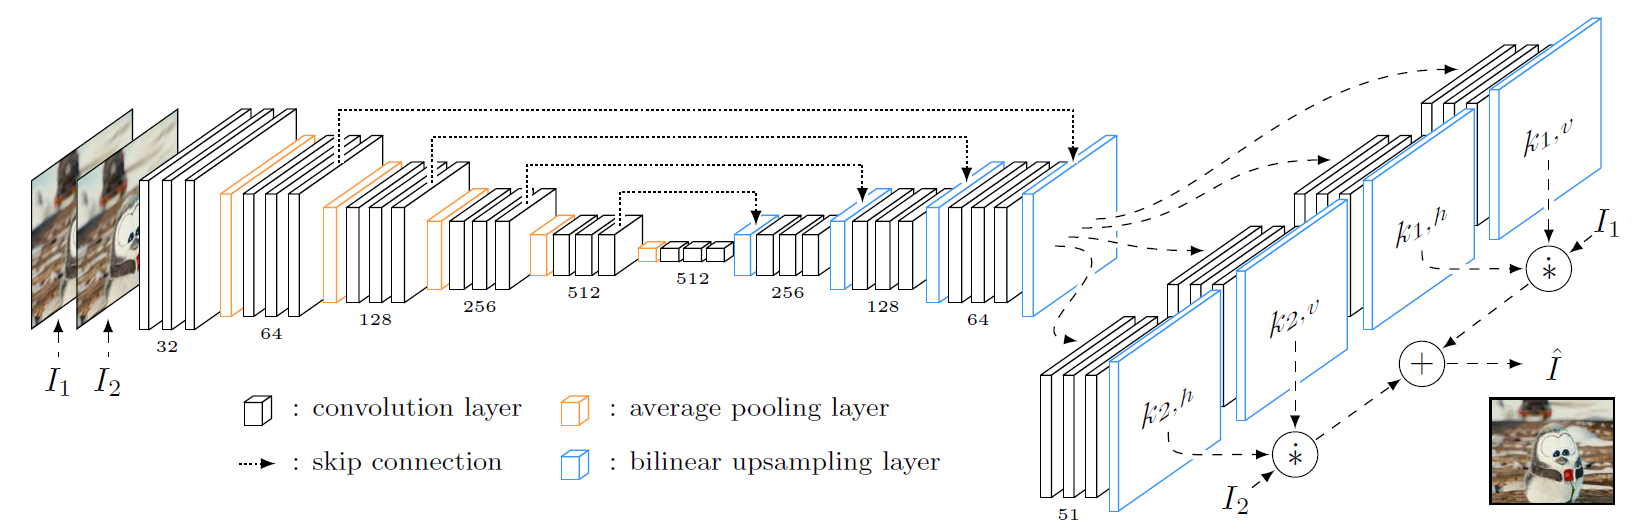
\includegraphics[width=0.6\textheight]{net_structure}
		\caption{Structure of original convolutional network. Note that $\dot{*}$ denotes a local convolution.}
		\label{original-net}
	\end{figure}

	\section{Experiment}
	In order to improve the performance of network we explored many solutions, some of which weren't useful and others were more interesting.\\
	Initially we maintained the original structure of the network, trying to change some parameters, but without significantly improvements. We tried:
	\begin{itemize}
		\item \textbf{Normalization:} we applied the normalization to the input images, calculating mean and variance, and for the last step we applied the denormalization, in order to obtain a better learning. That has proven ineffective, as dataset was already nearly normalized by its own;
		\item \textbf{Dropout:} the goal was improve performances and speed of network, but we don't observe noticeable difference in accuracy or computing time. Dropout helps to generalize what network is learning. We assume that this encoding-decoding architecture can generalize well enough that it doesn't need to dropout; 
		\item \textbf{Optimizer:} in CNN the most used optimization algorithm is Adam, so we used it for our experiments. We tested other optimization algorithms, like AdaMax or SDG, but without improvements.
	\end{itemize}
	Maintaining Adam as optimizer, without normalization and dropout, we tried to modify the structure of network and the loss function, to compare the results in \cite{mainpaper} with our loss functions.\\
	We applied two main changes to the network to get an improvement:
	\begin{itemize}
		\item we removed from every coding and decoding step a convolutional layer, transforming it from 3-stack to 2-stack convolutional layers. In this way, the time per epoch reduces by about 30\%, the network trains faster without the risk of under fitting;
		\item in the last step, when we apply the output network to the Equation~\ref{eq}, we added two additional convolution layers to see if the output image can be improved (e.g. sharpening it). 
	\end{itemize}
	Finally, we note that the network is able to overfit (if given enough epochs) even with large datasets, with 15-20 epochs this is avoided.
	
	\subsection{Loss functions}
	In \cite{mainpaper} the authors used two loss function: MSE and a perceptual loss, that is usually based on high-level features of images. They empirically found that the feature reconstruction loss based on the \texttt{relu4\_4}\footnote{\label{vgg-structure}To see the structure of VGG-19 with layer's name, visit \url{https://it.mathworks.com/help/deeplearning/ref/vgg19.html}} layer of the VGG-19 network produces good results for the frame interpolation task.\\
	Following the idea of using feature maps to create a loss function, we decided to try some other losses, therefore we used four different loss functions:
	\begin{itemize}
		\item \textbf{MSE}
		\item \textbf{VGG19-44}: we used the pretrained VGG-19 weights until layer \texttt{relu4\_4}. We use this loss because it focuses on the overall (local) appearance of the image. VGG-19 extracts features, focusing more on discriminative information (for classification) than e.g. noise;
		\item \textbf{VGG19-21}: we found that taking an earlier layer of the VGG-19 network, the \texttt{relu2\_1}\footref{vgg-structure}, gives a more interesting loss. At late layers the loss focuses on overall shapes, in this way our network matches harder the shape instead of its position on figures;
		\item \textbf{SobelKernel}: we created a mini network with two fixed convolutional layers with vertical and horizontal Sobel filters and then me compute MSE with the output. The idea is to focus more on maintaining the shape than on color information, to have less blurriness.
	\end{itemize}

	\subsection{Results}
	We execute the network with loss functions described above with the following parameters:
	\begin{itemize}
		\item \textbf{Size of dataset}: 50'000 examples, 128x128 pixels;
		\item \textbf{Batch size}: 32 examples;
		\item \textbf{Number of epochs}: 12;
		\item \textbf{Learning rate}: 0.001;
		\item \textbf{Kernel size}: 51 pixels;
		\item \textbf{Optimizer}: Adam.
	\end{itemize}
	To compare network's results we computed the \textit{Loss} and \textit{Peak Signal to Noise Ratio} (PSNR) metric, that measures in dB the quality of a reconstructed image. These metrics are computed for training, validation and test sets, called respectively: \textit{TrLoss, TrPS, VaLoss, VaPS, TeLoss} and \textit{TePS}.\\
	In Table~\ref{tab:old_results} we show performance of network described in the original paper \cite{mainpaper} and in Table~\ref{tab:results} we show the results of our network with modifies described above. In result's tables we report values only for the last epoch.\\
	Unfortunately, our results refer to a single execution of the network, because on average an epoch takes about 1000 seconds (using a graphic card with 8GB of VRAM). 

	\begin{table}
		\centering
		\begin{tabular}{|c|c|c|c|c|c|c|}
			\hline
			\textbf{LFunction} & \textbf{TrLoss} & \textbf{TrPS} & \textbf{VaLoss} & \textbf{VaPS} & \textbf{TeLoss} & \textbf{TePS}\\
			\hline
			MSE & 0.00462 & 71.59 & 0.0047 & 71.51 & 0.00475 & 71.46\\
			\hline
			VGG19-44 & 0.07695 & 69.48 & 0.07773 & 68.70 & 0.07794 & 68.68\\
			\hline
		\end{tabular}
		\caption{Performances of original network.}
		\label{tab:old_results}
	\end{table}

	\begin{table}
		\centering
		\begin{tabular}{|c|c|c|c|c|c|c|}
			\hline
			\textbf{LFunction} & \textbf{TrLoss} & \textbf{TrPS} & \textbf{VaLoss} & \textbf{VaPS} & \textbf{TeLoss} & \textbf{TePS}\\
			\hline
			MSE & 0.00495 & 71.28 & 0.00493 & 71.29 & 0.00498 & 71.26\\
			\hline
			VGG19-44 & 0.07468 & 68.64 & 0.07568 & 68.89 & 0.07594 & 68.84\\
			\hline
			%dati inventati per train e validation perché mancanti
			VGG19-21 & 0.005498 & 69.45 & 0.005941 & 70.74 & 0.005932 & 70.58\\
			\hline
			%dati inventati per train e validation perché mancanti
			SobelKernel & 0.01574 & 69.42 & 0.01763 & 69.51 & 0.01769 & 70.88\\
			\hline
		\end{tabular}
		\caption{Performances of our network.}
		\label{tab:results}
	\end{table}

	In Figure~\ref{output}, Figure~\ref{performance1} and Figure~\ref{performance2} we show network's outputs and graph's performance with different loss functions. All images show on top the original frames triplet and under the network's output frame. For \textit{SobelKernel} we show also the feature map of a network's output image and a label image.
	
	\vspace{0.5cm}
	Comparing the results in Table~\ref{tab:old_results} and Table~\ref{tab:results}, we observe that there isn't a significant difference between two architectures. Evidently, removing a convolutional layer from main structure or adding convolutional layers at the end of training doesn't improve performances or the generality of learning. The main difference is the speed of networks, because ours has about 17-18 millions of parameters, instead of other with about 20 millions of parameters.\\
	Comparing different loss functions, VGG19-21 has a lower loss than VGG19-21, probably because first loss function use weights that refer to a more high-level feature of images. However, comparing only Tables can be misleading, because seeing Figure~\ref{output} we note that every loss function highlight different features if images.\\ We saw that MSE output in Figure~\ref{out:our-mse} is blurry and on the contrary in Figure~\ref{out:our-vgg1944} and in Figure~\ref{out:vgg1921}, with VGG19 loss, the output is more sharper, but the network tends to replicate one of input frames.\\
	As last test, we used Sobel filter because it's faster than VGG loss and because it focuses on edges, so output images would remain defined. Unfortunately, the output in Figure~\ref{out:sobel} shows that SobelKernel loss doesn't improve the sharpness.\\
	We noted that with a smaller dataset, either using the SobelKernel loss or modifying the architecture with a single convolutional layer, we obtain significantly better results than with the standard net. Probably because with a large dataset, the network learns either more movements or shapes, hence it tents to insert them all in the output, creating a more blurred image.
	
	\begin{figure}
		\centering
		\subcaptionbox{Original network with MSE loss performances.\label{gr:or-mse}}{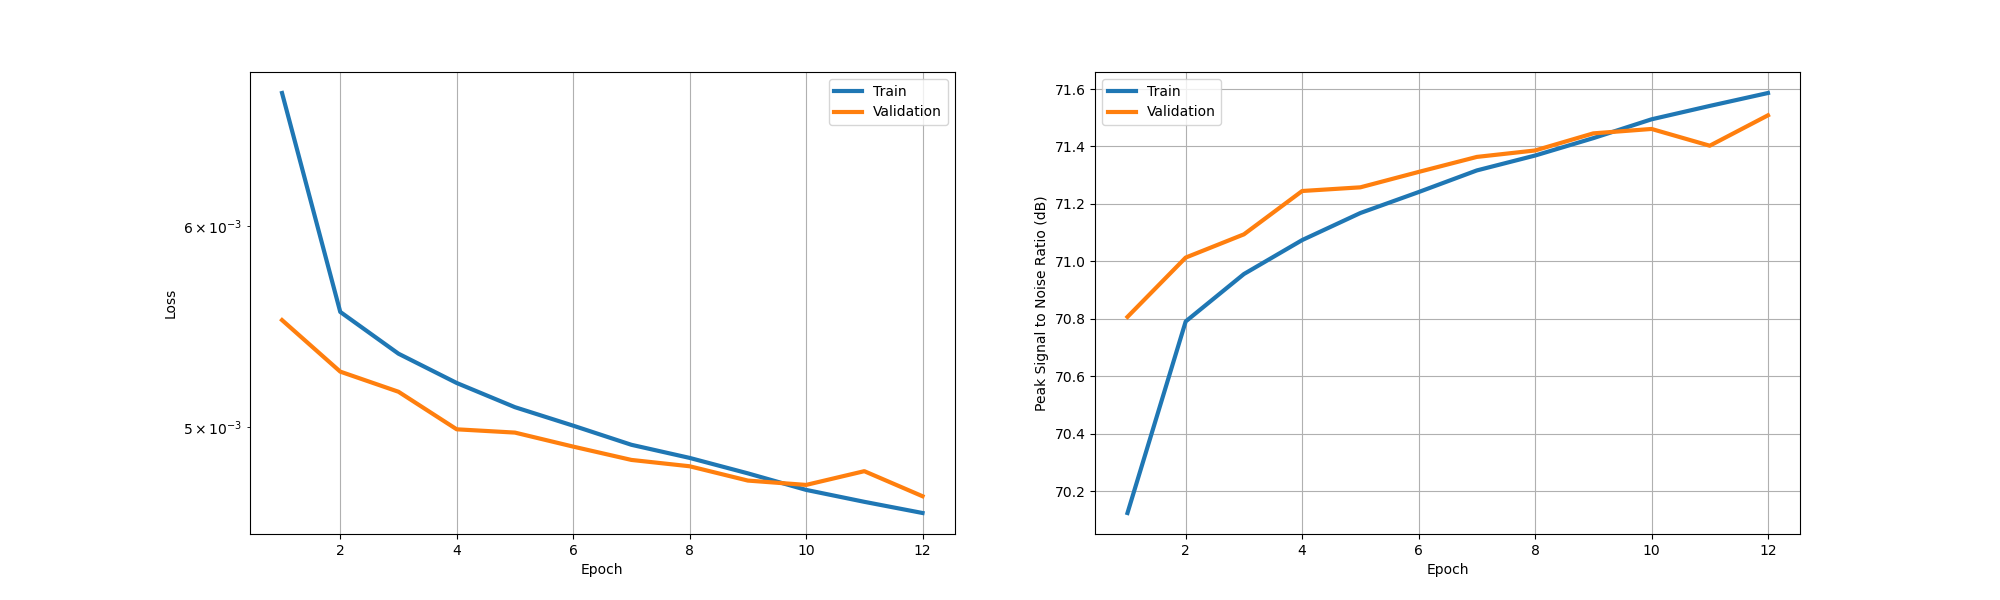
\includegraphics[width=0.7\textwidth]{orig_mse_graph}}
		\subcaptionbox{Our network with MSE loss performances.\label{gr:our-mse}}{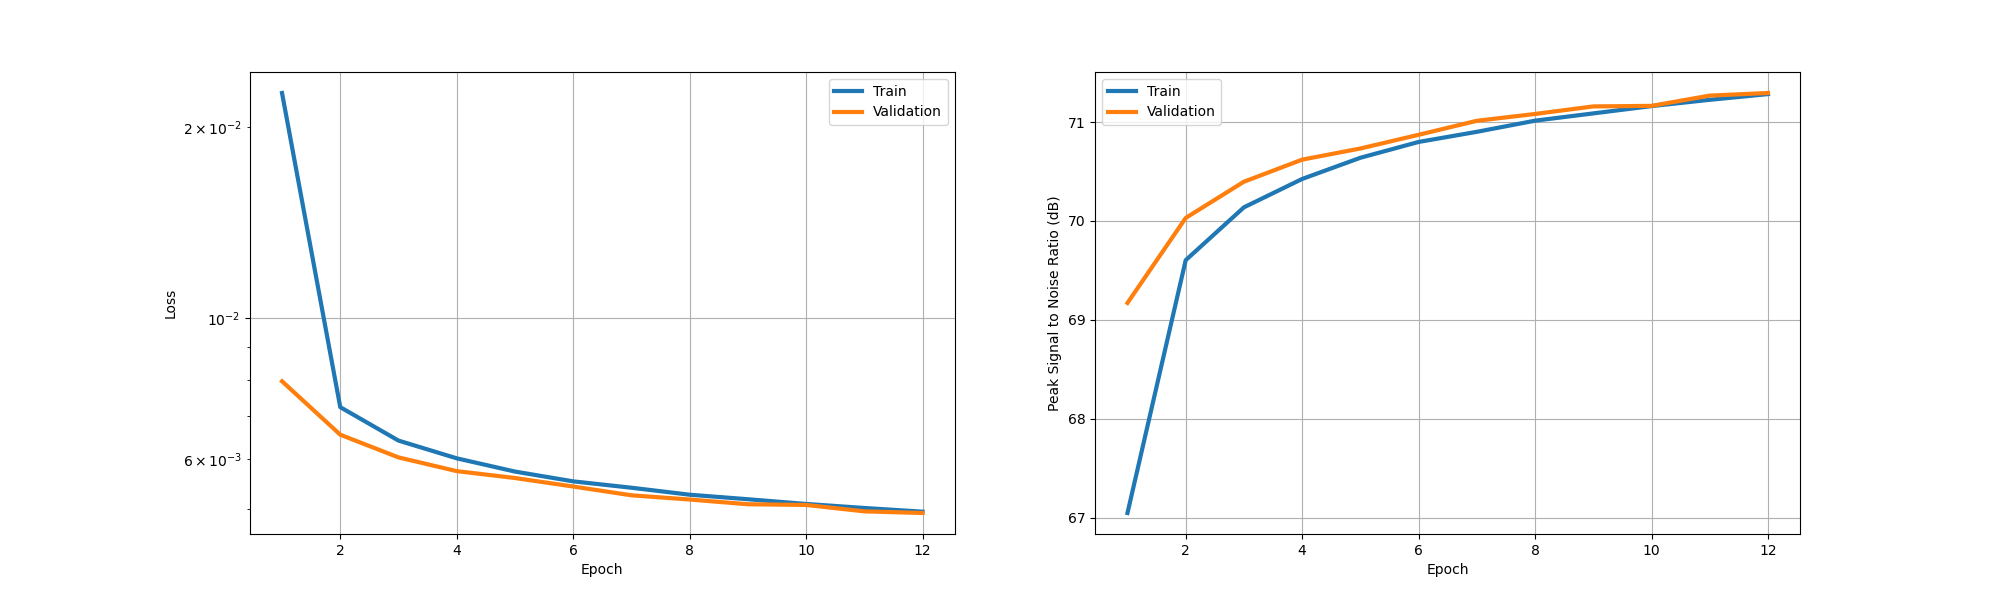
\includegraphics[width=0.7\textwidth]{our_mse_graph}}
		\subcaptionbox{Original network with VGG19-44 loss performances.\label{gr:or-vgg1944}}{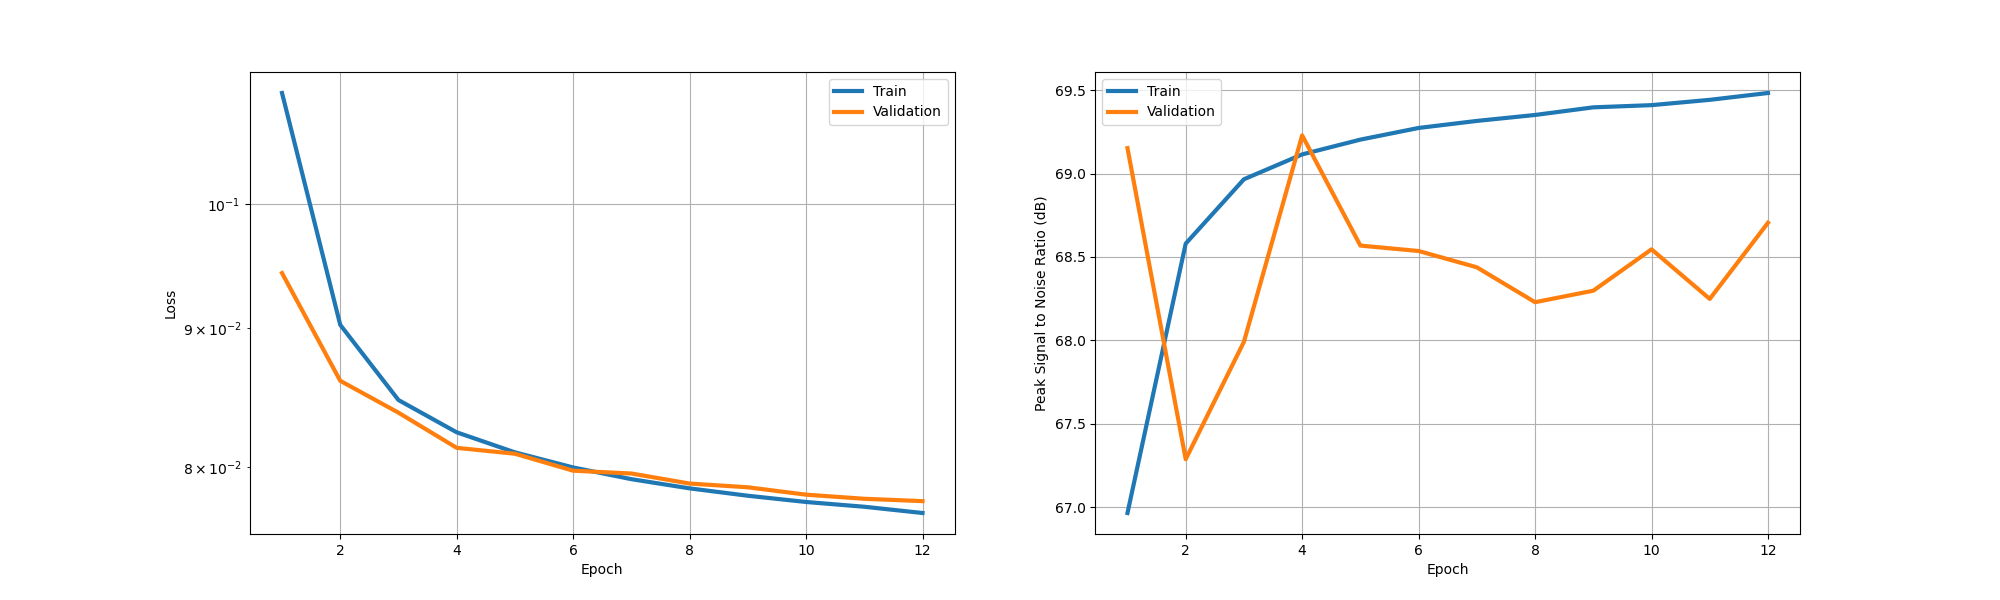
\includegraphics[width=0.7\textwidth]{orig_vgg19_44_graph}}
		\subcaptionbox{Our network with VGG19-44 loss performances.\label{gr:our-vgg1944}}{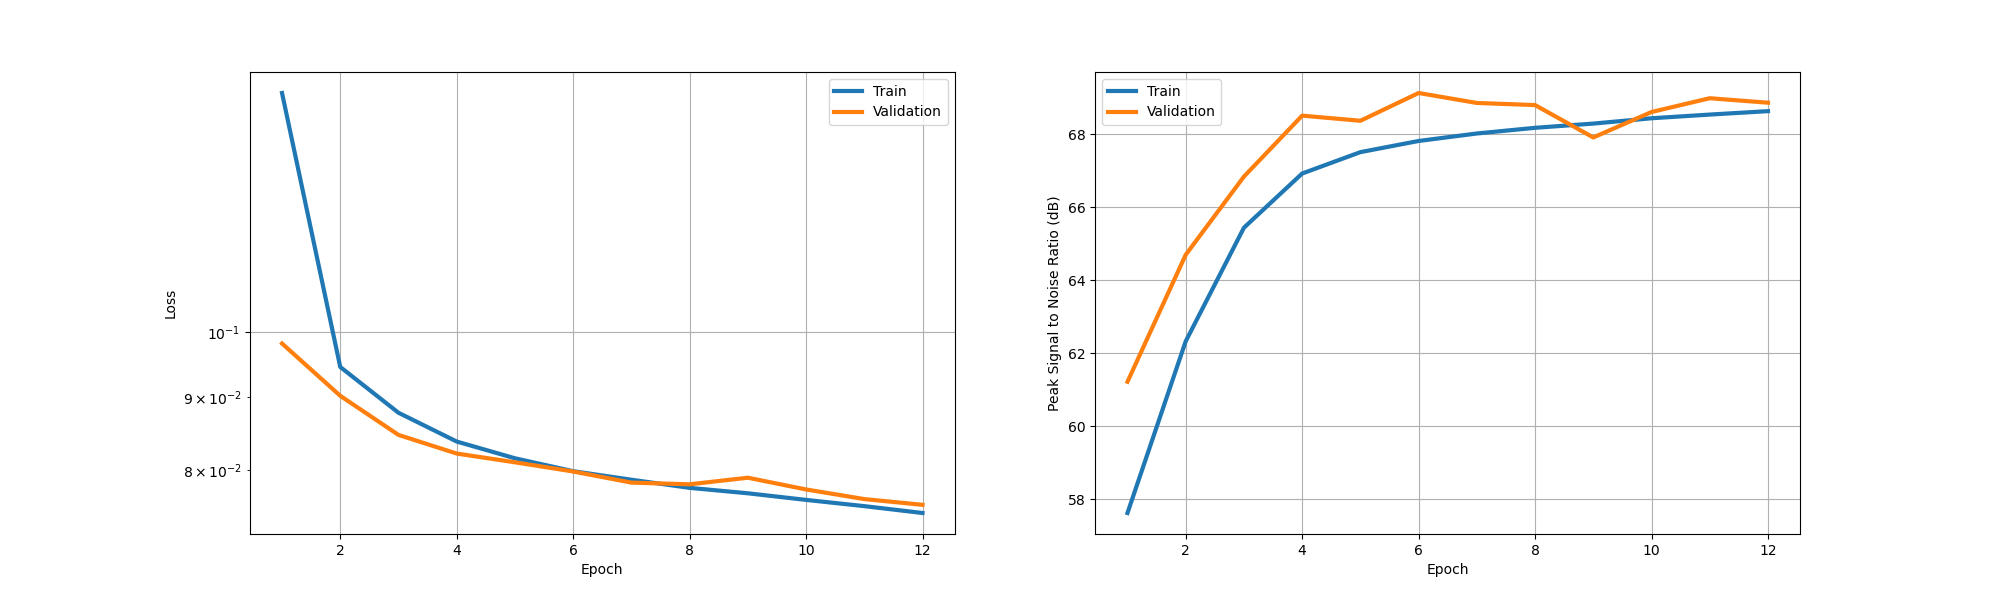
\includegraphics[width=0.7\textwidth]{our_vgg19_44_graph}}
		\subcaptionbox{Our network with VGG19-21 loss performances.\label{gr:vgg1921}}{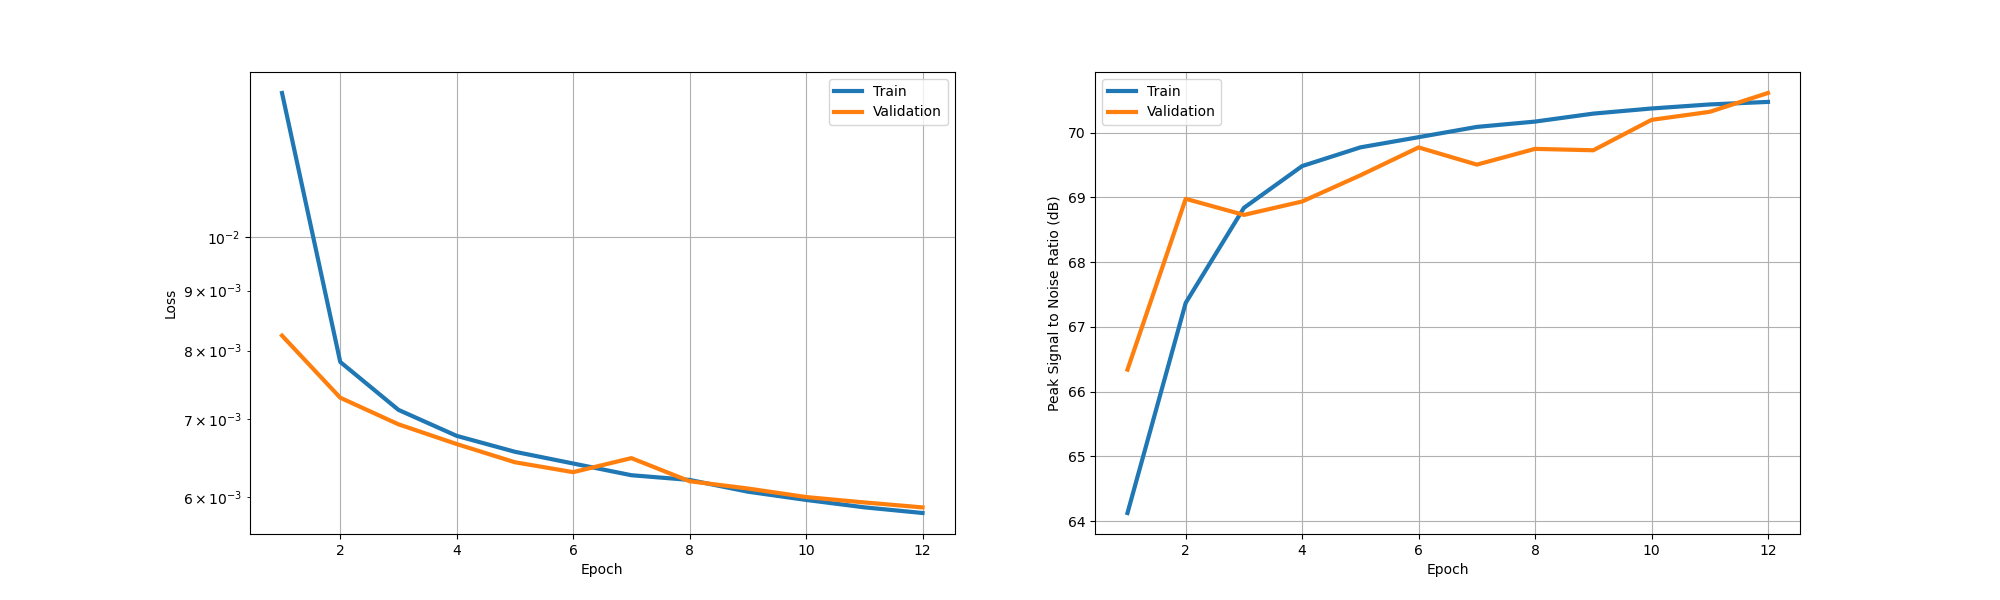
\includegraphics[width=0.7\textwidth]{vgg19_21_graph}}
		\subcaptionbox{Our network with SobelKernel loss performances.\label{gr:sobel}}{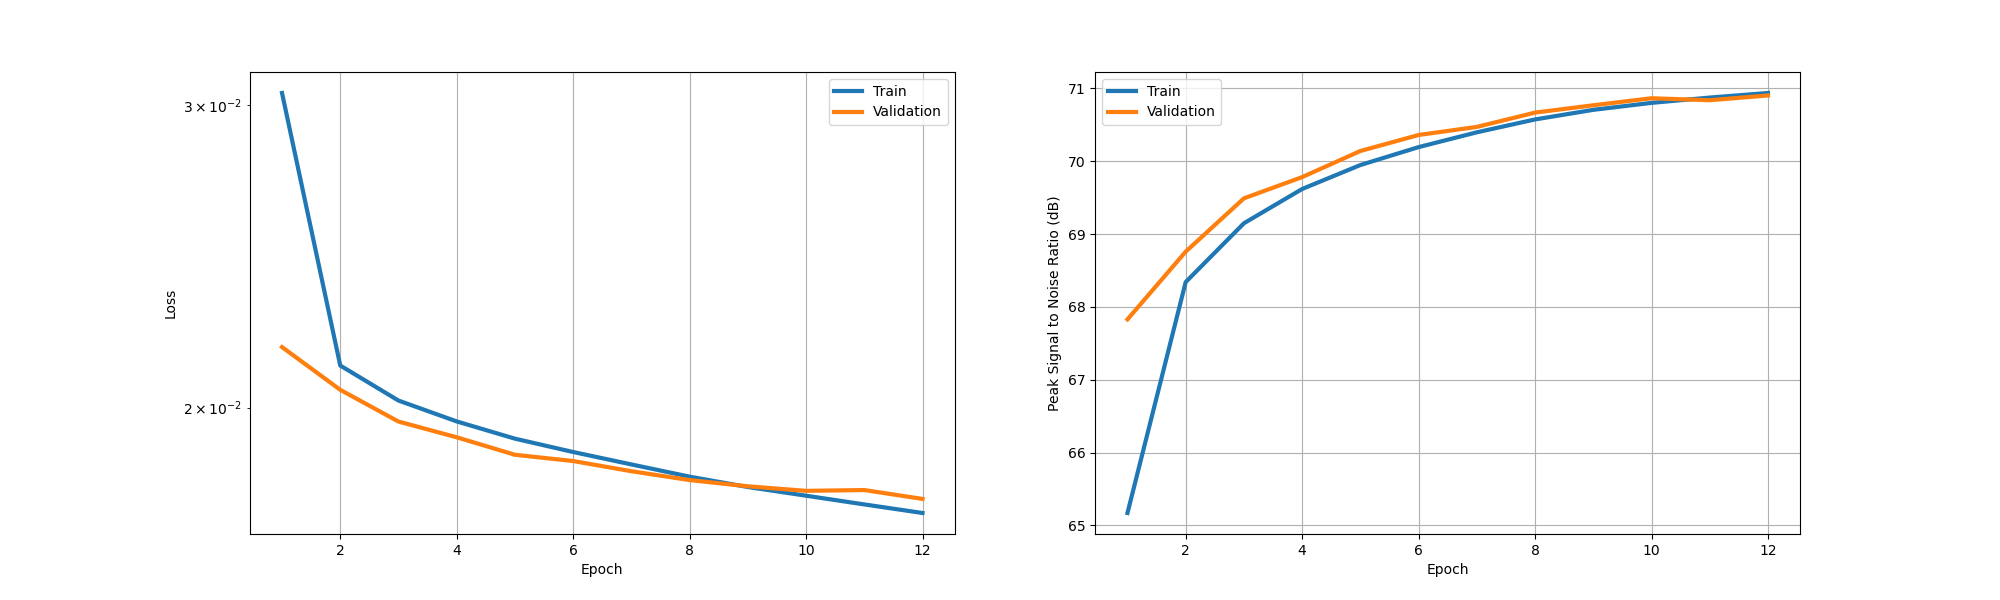
\includegraphics[width=0.7\textwidth]{sobel_graph}}
		\caption{Loss function's performances.}
		\label{performance1}
	\end{figure}
	\begin{figure}
		\centering
		\subcaptionbox{Early stage.}{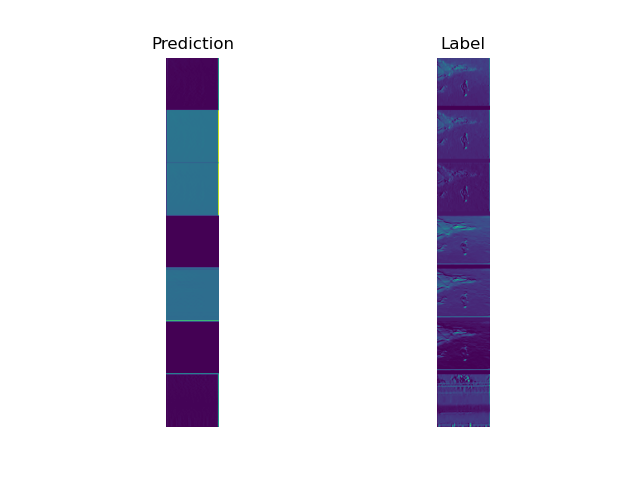
\includegraphics[width=0.3\textwidth]{sobel_map_1}}
		\subcaptionbox{Intermediate stage.}{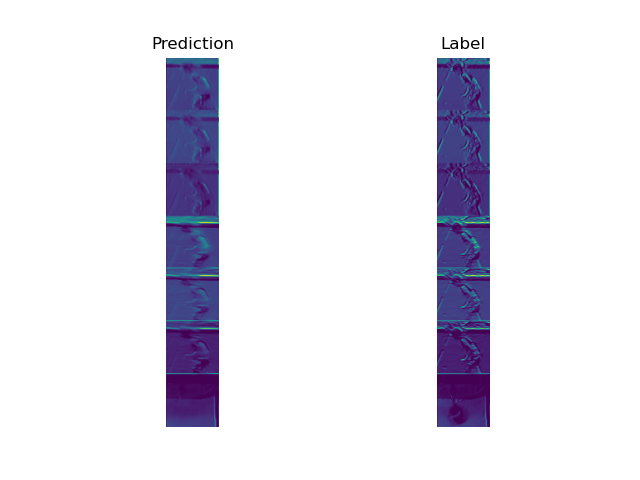
\includegraphics[width=0.3\textwidth]{sobel_map_2}}
		\subcaptionbox{Late stage.}{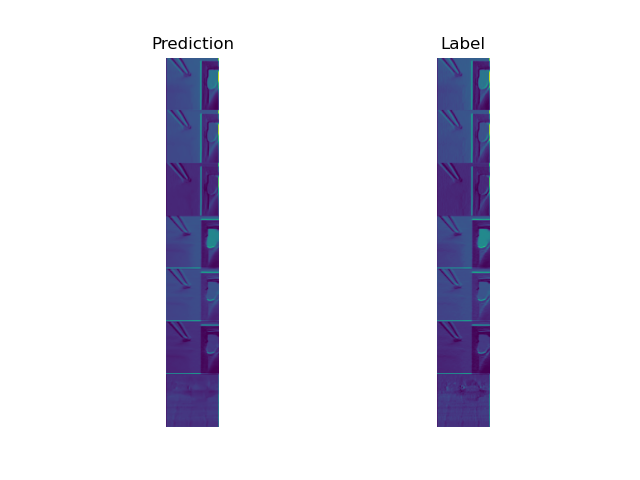
\includegraphics[width=0.3\textwidth]{sobel_map_3}}
		\caption{SobelKernel loss feature maps taken from different learning stages.}
		\label{performance2}
	\end{figure}

	\begin{figure}
		\centering
		\subcaptionbox{Output of original network with MSE loss.\label{out:or-mse}}{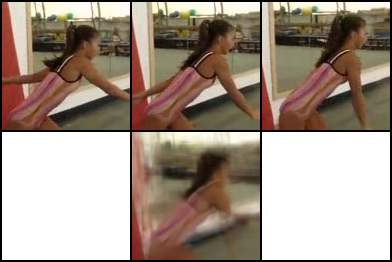
\includegraphics[width=0.45\textwidth]{orig_mse}}
		\subcaptionbox{Output of our network with MSE loss.\label{out:our-mse}}{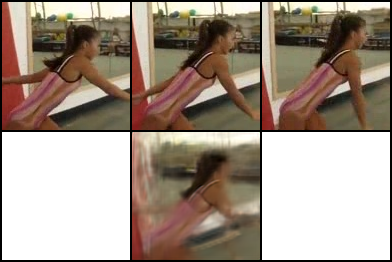
\includegraphics[width=0.45\textwidth]{our_mse}}
		\subcaptionbox{Output of original network with VGG19-44 loss.\label{out:or-vgg1944}}{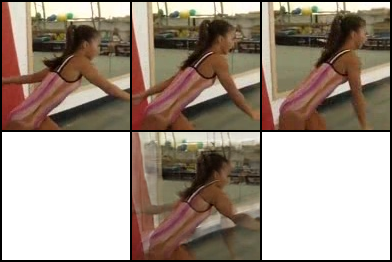
\includegraphics[width=0.45\textwidth]{orig_vgg19_44}}
		\subcaptionbox{Output of our network with VGG19-44 loss.\label{out:our-vgg1944}}{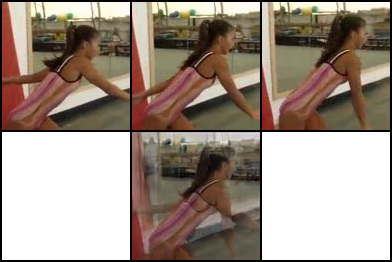
\includegraphics[width=0.45\textwidth]{our_vgg19_44}}
		\subcaptionbox{Output of out network with VGG19-21 loss.\label{out:vgg1921}}{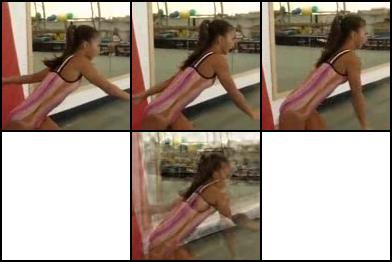
\includegraphics[width=0.45\textwidth]{vgg19_21}}
		\subcaptionbox{Output of our network with SobelKernel loss.\label{out:sobel}}{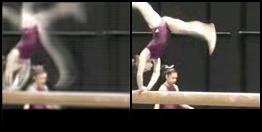
\includegraphics[width=0.45\textwidth]{sobel}}
		\caption{Network's outputs.}
		\label{output}
	\end{figure}
	
	
	\subsection{Dvd Logo}
	As mentioned above, testing our network with with VGG-19 filters, we saw that the interpolated frames tended to be identical to one of two input frames. To test if the network actually learns the translation of figures in an image, we tested the network with a video that shows a single object that make a translation (the simplest movement), like this \href{https://www.youtube.com/watch?v=5mGuCdlCcNM}{Youtube video}.\\
	As result, we see in Figure~\ref{dvd} that using a simple dataset, the network can actually learn the movements of figures in the video; probably a great help is given by a well defined background. 
	
	\begin{figure}
		\centering
		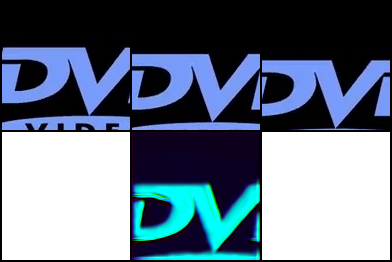
\includegraphics[width=0.45\textwidth]{dvd1}
		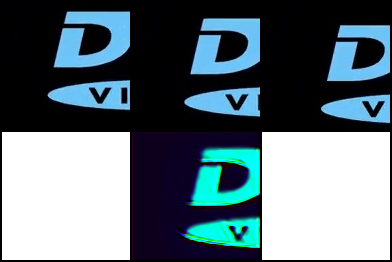
\includegraphics[width=0.45\textwidth]{dvd2}
		\caption{Translation of a figure}
		\label{dvd}
	\end{figure} 
	
	\section{Conclusion}
	Changing the network architecture we don't earn better performance, but trying different loss functions we could observe that the combination of frames is done differently, mainly blurring them together, choosing a frame or an hybrid of the 2 things.\\ 
	The video frame interpolation task can also help for action recognition task in the pretrain phase, in case we want to elaborate more detailed movements.
	
	\bibliographystyle{unsrt}
	\bibliography{bibliography}
	
\end{document}